\documentclass[letterpaper,twocolumn,10pt]{article}
\usepackage{usenix-2020-09}
\usepackage[T1]{fontenc}
\usepackage[utf8]{inputenc}
\usepackage{graphicx}
\usepackage{booktabs}
\usepackage{enumitem}
\usepackage{hyperref}

\Urlmuskip=0mu plus 1mu

\title{\Large CS-412 Software Security Fuzzing Lab\\Fuzzing \texttt{libpng} with AFL++}

\author{
Group 7\\
EPFL --- Spring 2026
}

\date{}

\begin{document}
\maketitle

\begin{abstract}
We fuzz \texttt{libpng} 1.2.56 with AFL++ in three configurations:
source-instrumented with ASan, AFL-instrumented without ASan, and QEMU
mode against a vanilla \texttt{gcc} build. The decoder harness drives
\texttt{png\_read\_info}, transforms, \texttt{png\_read\_image}, and
\texttt{png\_read\_end} on ten small PNG seeds with the AFL++ PNG
dictionary and a CRC-neutralised libpng. The 32-minute instrumented run
reaches 966 of 3{,}122 edges (30.94\% bitmap) and saturates locally; a
text-API harness reproduces a CVE-2016-10087-style heap-buffer-overflow
in \texttt{png\_set\_text\_2}. We use the QEMU and persistent runs to
discuss the limits of edge-count and bitmap comparisons across
instrumentation sources.
\end{abstract}

\section{Setup and Methodology}
\textbf{Target and environment.}
The target is \texttt{libpng} 1.2.56, built inside the provided Ubuntu 24.04 Docker environment. The image builds AFL++, downloads the \texttt{v1.2.56} libpng source, applies our CRC-neutralization patch, and installs three static library variants: AFL++ instrumentation with ASan, AFL++ instrumentation without ASan, and a vanilla \texttt{gcc} build for QEMU mode. The harnesses are in \texttt{src/}; the main decoder harness is \texttt{harness.c}, the persistent variant is \texttt{harness\_persistent.c}, and the focused API harnesses are \texttt{harness\_text\_api.c}, \texttt{harness\_write\_api.c}, and \texttt{harness\_metadata\_api.c}.

\textbf{Campaigns and artifacts.}
The baseline decoder campaigns ran for approximately 32 minutes in source-instrumented ASan mode and QEMU mode. Longer supporting campaigns were also run for the persistent decoder and for the write, metadata, and text API harnesses; their compact evidence is kept under \texttt{triage-artifacts/}. Plots generated with \texttt{afl-plot}, minimized crash inputs, ASan traces, and final AFL++ status metrics are referenced in the appendix once the Person 1 and Person 2 evidence packets are finalized.

\section{Evaluation Questions}
\noindent\textit{Each subsection corresponds to one graded question.}

\subsection{Q1 --- Harness Design}
The primary fuzz target is the explicit read pipeline rather than a wrapper such as \texttt{png\_read\_png()}. AFL++ passes a testcase path through \texttt{@@}; the harness reads that file into an \texttt{InputState} buffer and gives libpng a custom \texttt{png\_set\_read\_fn()} callback. The callback copies exactly the number of bytes requested by libpng and raises \texttt{png\_error()} on out-of-input reads. This models a normal stream while keeping the testcase deterministic and avoiding interactive or OS-dependent behavior.

After creating \texttt{png\_struct} and \texttt{png\_info}, the harness installs \texttt{setjmp(png\_jmpbuf(...))} so ordinary malformed PNGs return cleanly instead of terminating the fuzzer. It then executes \texttt{png\_read\_info()}, applies common transforms with \texttt{png\_set\_expand()}, \texttt{png\_set\_strip\_16()}, \texttt{png\_set\_gray\_to\_rgb()}, background handling, and gamma correction, calls \texttt{png\_read\_update\_info()}, allocates row buffers, reaches \texttt{png\_read\_image()}, and finishes with \texttt{png\_read\_end()}. This path covers signature checks, chunk parsing, zlib inflation, filtering, interlacing-related row logic, and color conversion decisions.

The main resource guard rejects images wider or taller than 4096 pixels before row allocation. This does not try to validate PNG semantics; it only prevents AFL++ from spending time or memory on huge allocations that are unlikely to improve bug-finding. Cleanup is centralized so both success and libpng error paths free row buffers, destroy libpng state, close the file, and release the input buffer. The persistent harness preserves the same decoding logic but wraps it in \texttt{\_\_AFL\_LOOP(1000)} to measure forkserver overhead separately in Q8.

We also added focused API harnesses because the full decoder does not naturally exercise all public setter paths. The text API harness directly targets \texttt{png\_set\_text()} twice, with fuzz-controlled keys, text pointers, compression mode, and optional \texttt{png\_free\_data()}; this is the harness that exposed the confirmed text finding. The metadata API harness drives setters for color, physical, profile, time, and unknown-chunk metadata. The write API harness creates synthetic image rows and exercises \texttt{png\_create\_write\_struct()}, output callbacks, row writing, filters, compression options, palette mode, bit-depth choices, and transform flags. These harnesses complement the decoder rather than replacing it.

\subsection{Q2 --- Instrumentation and Sanitizers}
The source-instrumented build uses \texttt{afl-clang-fast} with \texttt{-fsanitize=address -g -O1}; the harness links statically against \texttt{/build/install/lib/libpng12.a} with \texttt{-fsanitize=address -lz -lm}. ASan turns heap overflows, use-after-free, and many invalid accesses into deterministic crashes that AFL++ can save. The runtime sets \texttt{ASAN\_OPTIONS} to abort on errors, disable leak detection, and skip inline symbolization; this makes sanitizer findings visible to AFL++, avoids leak noise in fuzzing loops, and leaves stack symbolization to triage.

For QEMU mode, the target is rebuilt with \texttt{gcc -g -O1}, no sanitizer, and no AFL++ compile-time counters, then run with \texttt{afl-fuzz -Q}. This simulates a binary-only target and measures the cost of dynamic translation and runtime coverage collection. For Q8, a third library variant is built with \texttt{afl-clang-fast -g -O1} but without ASan, allowing a same-harness comparison of sanitizer overhead versus fork/persistent execution overhead.

The key source patch is \texttt{patches/libpng-1.2.56-no-crc.patch}, which changes \texttt{pngrutil.c}'s CRC check in \texttt{png\_crc\_finish()} to always report success. PNG chunks carry CRC-32 checksums; normal byte-level mutations almost immediately invalidate them. Without the patch, libpng rejects critical chunks early or discards mutated ancillary chunks, so AFL++ receives little feedback from deep parsers. With CRC neutralized, mutated chunk contents continue into chunk-specific code, decompression, transform setup, and metadata handling. The tradeoff is that the campaign no longer measures behavior behind strict CRC validation; for this lab that is acceptable because the objective is to reach security-relevant parsing code.

\subsection{Q3 --- Seed Corpus and Dictionary}
Havlin:
The decoder seed corpus intentionally uses small, valid PNGs with structural diversity rather than large photographs. The ten decoder seeds cover RGB, RGBA, grayscale with transparency, indexed color with PLTE, 16-bit grayscale, grayscale+alpha, ancillary text, an iTXt/CVE-oriented sample, Adam7 interlacing, and a multi-IDAT/hIST case. This gives AFL++ valid signatures, chunk ordering, dimensions, color modes, and metadata examples while keeping mutation cost low.

The API harnesses use separate small textual seed corpora because their inputs are not PNG files; they are byte layouts interpreted by the harnesses as selectors, lengths, flags, strings, palette data, metadata values, and row-generation parameters. This keeps the fuzzer close to the public API state we want to test instead of requiring it to discover those states through a complete PNG file.

For the decoder campaigns we pass the AFL++ PNG dictionary with \texttt{-x /build/dictionaries/png.dict}. In language terms, PNG files are not arbitrary byte strings; they follow a grammar consisting of the fixed PNG signature followed by chunks of the form length, type, data, CRC. Dictionary tokens such as the signature and chunk-type terminals \texttt{IHDR}, \texttt{PLTE}, \texttt{IDAT}, \texttt{IEND}, \texttt{tEXt}, \texttt{zTXt}, and \texttt{iTXt} bias AFL++ insertions and replacements toward syntactically meaningful regions of that grammar. The dictionary does not replace coverage guidance, but it increases the chance that havoc and splice mutations preserve or create recognizable chunk boundaries.

% TODO(P2): Add concrete AFL++ yield evidence for dictionary/havoc/splice here.
The final report should add the observed AFL++ mutation-yield numbers for dictionary, havoc, and splice once the campaign evidence owner extracts them from the final status screens or \texttt{fuzzer\_stats}. Those numbers should be interpreted as support for the seed/dictionary strategy, not as standalone proof of correctness.


The campaign starts from ten small valid PNGs in \texttt{seeds/} (69--1388
bytes, 3909 bytes in total). They cover RGB, RGBA, greyscale, greyscale+alpha,
16-bit greyscale, indexed colour with \texttt{PLTE} and \texttt{tRNS}
transparency, \texttt{iTXt} text metadata, Adam7 interlacing, and
multi-\texttt{IDAT}/\texttt{hIST} cases. The point of keeping them small is
that AFL++ calibrates and mutates each seed many times per second, so wasted
bytes are wasted budget. The point of the diversity is that each seed already
sits past the PNG signature and IHDR gate in a different state, so havoc
mutation immediately exercises palette handling, ancillary chunks, zlib
decompression, and scanline filters instead of having to first invent a valid
container from random bytes.

All reader campaigns add the AFL++ PNG dictionary with
\texttt{-x /build/dictionaries/png.dict}. The Docker image copies it from the
AFL++ distribution and the Makefile exposes it as \texttt{PNG\_DICT}. The
useful entries are the PNG signature and the four-byte chunk type tokens
(\texttt{IHDR}, \texttt{PLTE}, \texttt{IDAT}, \texttt{IEND}, \texttt{tRNS},
\texttt{gAMA}, \texttt{tEXt}, and others). PNG is a binary grammar of the
shape \(\mathit{File} \to \mathit{Signature}\ \mathit{Chunk}^{+}\) where each
chunk is \texttt{length / type / data / CRC}. The dictionary gives AFL++ the
terminal tokens for the signature and the type field; chunk ordering, lengths, 
CRCs, filter bytes, and compressed IDAT payloads are all semantic structure the 
mutator then discovers through coverage feedback.

For the per-strategy yield numbers we needed AFL++'s live status rows, which
the fuzzer does not write to \texttt{fuzzer\_stats} or \texttt{plot\_data}. We
captured them from two short 300~s supplementary runs and preserved the
transcripts and an extracted summary in \texttt{evidence/q3-live/}. The first
run kept deterministic stages on (13{,}109 execs, 804 edges) so the
dictionary row would actually fill in; the second used \texttt{-z -u} to skip
deterministic stages and reach havoc/splice fast enough inside the 300~s
budget (12{,}650 execs, 721 edges). These are evidence runs for Q3, not the
canonical Q4 campaign.

\begin{table}[h]
\centering
\small
\begin{tabular}{lrrr}
\toprule
\textbf{Strategy} & \textbf{Finds} & \textbf{Attempts} & \textbf{Yield} \\
\midrule
Dictionary overwrite & 55 & 2{,}726 & 2.02\% \\
Dictionary insert & 0 & 2{,}754 & 0.00\% \\
Havoc & 61 & 6{,}500 & 0.94\% \\
Splice & 4 & 420 & 0.95\% \\
\bottomrule
\end{tabular}
\caption{AFL++ strategy yields from the live status captures.}
\end{table}

Dictionary \emph{overwrite} is the high-precision, low-volume operator: it
replaces a few existing bytes with a known token, so a malformed four-byte
chunk type can flip in one mutation to something the parser recognises and
advance to the next validation or decompression stage. That is why it
delivers the best yield (2.02\%). Dictionary \emph{insert} is the same
operation without the alignment constraint, and on PNG it spends its budget
breaking chunk lengths; in this run it found nothing in 2{,}754 attempts.
Havoc is lower precision but higher volume: stacked random flips, overwrites,
insertions, deletions, and size changes mostly break chunk alignment or
compressed data, but 6{,}500 attempts give the mutator plenty of chances to
land on a useful perturbation of dimensions, filter bytes, or payloads, which
explains 61 finds at a 0.94\% yield. Splice has the highest variance because
gluing two PNG inputs together usually leaves IHDR, PLTE, and IDAT
inconsistent with each other, but a clean chunk-boundary recombination can
still expose a new parser state -- 4 finds in 420 attempts is what that looks
like in practice.

\subsection{Q4 --- Campaign Analysis}
The Q4 run we use is the ASan source-instrumented decoder campaign on the
ten PNG seeds with the PNG dictionary, target \texttt{./png\_fuzz}. Its
final \texttt{fuzzer\_stats} counters are:

\begin{table}[h]
\centering
\small
\begin{tabular}{lr}
\toprule
\textbf{Metric} & \textbf{Value} \\
\midrule
Executions / speed & 1{,}034{,}958 / 532.08 exec/s \\
Corpus count & 715 files \\
Cycles done & 5 \\
Stability & 100.00\% \\
Bitmap coverage & 30.94\% \\
Edges found / total & 966 / 3{,}122 \\
Crashes / hangs & 0 / 2 \\
\bottomrule
\end{tabular}
\end{table}

Stability is 100\% and AFL++ recorded zero variable corpus entries, so the
harness ran deterministically. That does not prove bug absence, but it does
mean the two saved hangs are real timeout candidates worth triage rather than
fuzzer noise. The queue grew from 10 seeds to 715 files (a 71.5$\times$
expansion), and AFL++ only keeps mutations that add coverage, so that growth
reflects the seed set crossing the signature, IHDR, palette, interlace, and
ancillary-chunk gates and then expanding inside each of those regions.

The \texttt{plot\_data} edge curve has the standard fast-rise, slow-tail
shape: 735 edges at 61~s, 876 at 325~s, slowing from roughly 0.53 to
0.067 edges/s between 325~s and the last find at 1{,}677~s (966 edges), then
flat for 268~s to the end of the run. That tail is local saturation: AFL++
has exhausted the easy-to-reach paths for \emph{this} harness, seed set,
dictionary, CRC-neutralised build, and ASan fork-mode budget. It is not
evidence that libpng has been fully explored. 966 reached edges out of
3{,}122 instrumented edges is 30.94\%, so the majority of the instrumented
explore space is still untouched. Most of what remains is gated by semantic
constraints (specific chunk ordering, transform combinations, IDAT inflate
states) and by API surfaces that are not called in the decoder harness.

The longer parallel campaigns confirm rather than overturn this. Six
persistent decoder workers ran for $\sim$21{,}593~s and summed to
565{,}639{,}982 execs at 26{,}194 exec/s, reaching 1{,}088 / 3{,}131 edges
(34.75\% bitmap); the main worker's last edge landed at 19{,}220~s and
then stayed flat until 21{,}596~s. Its two saved crash files are
low-confidence: standalone ASan replay did not reproduce either, and
main-worker stability sat at 99.91\%, leaving room for fuzzer-environment
non-determinism or cross-iteration state leak. Write-API: 35{,}705{,}101
execs, 558 / 2{,}090 edges, last find at 194~s -- a narrow encoder-facing
state space under our seeds. Metadata-API: 31{,}283{,}024 execs,
458 / 3{,}388 edges (13.52\%), zero crashes or hangs -- negative evidence
for that harness, not proof. For all three, \texttt{afl-plot} renders only
the main worker; campaign-wide totals come from summing per-worker
\texttt{fuzzer\_stats}.

\subsection{Q5 --- Crash Triage (0--5 points)}
\textbf{What to answer.}
\begin{itemize}[leftmargin=*]
  \item If crashes found: reproduce, minimize with \texttt{afl-tmin}, collect ASan trace, identify bug class and possible CVE.
  \item If no crashes: inject synthetic bug, fuzz for 60s, show detection, then justify why no real bugs were found.
\end{itemize}
\textbf{Example angle from handout.}
\begin{itemize}[leftmargin=*]
  \item Workflow: reproduce \(\rightarrow\) minimize \(\rightarrow\) ASan diagnosis with command/output evidence.
\end{itemize}
\textbf{Your content.} % include command snippets and observed output summary

\subsection{Q6 --- Attack Surface Analysis}
Two realistic consumers of libpng are Firefox and ImageMagick. Firefox's PNG decoder lives in \texttt{image/decoders/nsPNGDecoder.cpp}: it includes \texttt{png.h}, creates libpng read state, configures unknown chunks and limits, and uses progressive callbacks through \texttt{png\_set\_progressive\_read\_fn()}.\footnote{\url{https://searchfox.org/firefox-main/source/image/decoders/nsPNGDecoder.cpp}} ImageMagick's PNG coder lives in \texttt{coders/png.c}: it contains read and write entry points such as \texttt{ReadPNGImage()}, \texttt{ReadOnePNGImage()}, and \texttt{WritePNGImage()}, and calls libpng through application-specific blob I/O, options, profile handling, and MNG/JNG support.\footnote{\url{https://github.com/ImageMagick/ImageMagick/blob/main/coders/png.c}}

In a browser scenario, an attacker can place a malicious PNG in a web page, favicon, CSS image, downloaded attachment preview, or image cache path. The exposed surface is not only libpng's core chunk parser; it is the complete browser image pipeline around progressive network input, metadata decode, color management, frame allocation, and surface output. A memory corruption in that path could at minimum crash the content process and, depending on sandboxing and exploitability, become part of a renderer compromise chain. In an ImageMagick scenario, a server may call \texttt{identify}, \texttt{convert}, or a library binding on user-uploaded images to generate thumbnails or metadata. A crafted PNG can then reach a long-running backend process, where denial of service is already relevant and memory corruption can be more serious if the service has access to stored media or internal files.

Our harnesses cover important libpng behavior, but they are not full application harnesses. First, Firefox uses progressive decoding: \texttt{nsPNGDecoder::InitInternal()} installs \texttt{info\_callback}, \texttt{row\_callback}, and \texttt{end\_callback}, while \texttt{ReadPNGData()} feeds chunks incrementally and handles libpng \texttt{setjmp} errors. Our decoder harness instead calls the sequential \texttt{png\_read\_info()} / \texttt{png\_read\_image()} API on a complete in-memory input. This misses browser-specific streaming states, pause/resume transitions, and callback ordering. Firefox also parses PNG eXIf data with \texttt{EXIFParser::Parse()}, uses qcms color transforms, and has APNG frame paths such as \texttt{frame\_info\_callback()}; none of those application-level paths are exercised by our standalone decoder.

Second, ImageMagick wraps libpng with substantial logic that our harnesses do not model. \texttt{ReadOnePNGImage()} handles ImageMagick blob I/O, resource limits, raw profile extraction from text chunks via \texttt{Magick\_png\_read\_raw\_profile()}, user options such as CRC handling and ICC-profile preservation, and conversion into ImageMagick's pixel cache. \texttt{ReadMNGImage()} and \texttt{ReadOneJNGImage()} add multi-image and JPEG-in-PNG-family formats that are outside our PNG-only decoder. Even though our write API harness calls libpng's write-side functions, it does not cover ImageMagick's \texttt{WritePNGImage()} path, where input comes from ImageMagick image objects, quantization/depth-reduction choices, profiles, and format-specific command options. These gaps matter because application glue often creates the exact state combinations, allocators, and lifetime patterns that isolated library harnesses intentionally simplify away.

\subsection{Q7 --- Binary-Only Fuzzing with QEMU}
% TODO(P2): Add equal-wall-clock ASan fork vs QEMU table and QEMU-long note.
The QEMU comparison should use the roughly equal 32-minute ASan fork and QEMU short decoder runs as the clean side-by-side experiment. The longer QEMU run lasted about 3 hours 39 minutes and should be mentioned only as supporting evidence, not as a clean 6-hour comparison. The explanation should distinguish compile-time AFL++ edge counters from QEMU's dynamic translation and runtime coverage collection, and should compare exec speed, edges discovered, and corpus size.

\subsection{Q8 --- Instrumentation Depth and Performance}
% TODO(P2): Add edge-count measurements and same-machine three-way speed table.
The final Q8 section should report instrumented edge counts for libpng alone and for the final harness binary, then compare no-sanitizer fork mode, ASan fork mode, and ASan persistent mode on the same machine and seed corpus. The expected interpretation is that ASan slows each execution by adding memory checks and redzones, while persistent mode removes much of the process creation overhead by reusing one initialized process across many AFL++ iterations.

\section{Conclusion}
The harness design reached the intended libpng decoder surface and the focused API harnesses expanded coverage beyond file parsing into public setter and writer APIs. The strongest confirmed result so far is the text API finding; the main remaining work is evidence polish: final plots and speed measurements, a minimized ASan trace, and a careful distinction between confirmed bugs, pending hangs, and excluded harness artifacts.

\appendix
\section{Appendix: Evidence and Figures}
\begin{figure}[h]
\centering
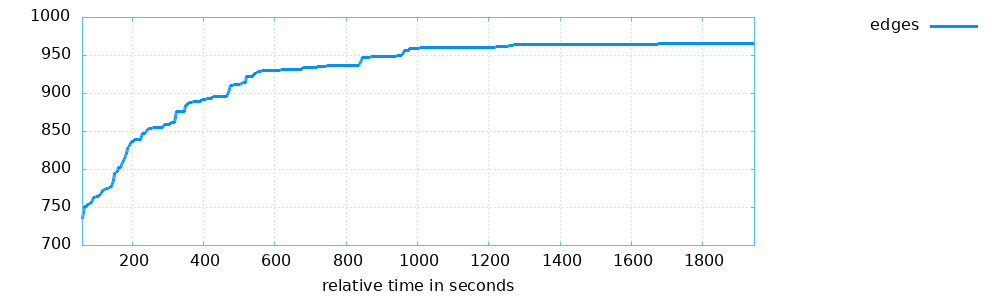
\includegraphics[width=\linewidth]{plot_output/edges.png}
\caption{Baseline source-instrumented decoder edges over time. Replace or keep after Person 2 finalizes the selected plot set.}
\end{figure}

\begin{figure}[h]
\centering
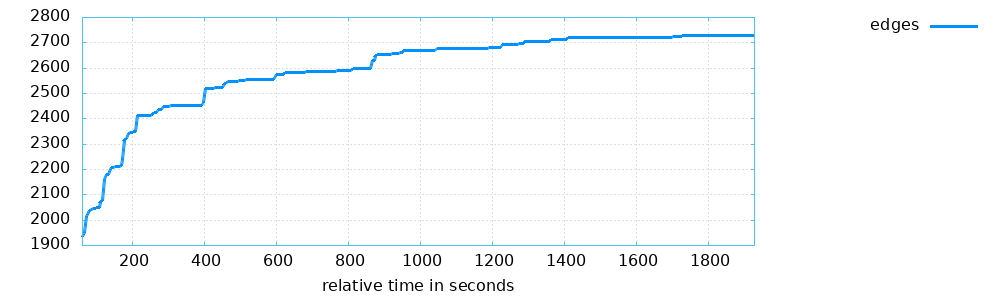
\includegraphics[width=\linewidth]{plot_output_qemu/edges.png}
\caption{Baseline QEMU decoder edges over time. Replace or keep after Person 2 finalizes the selected plot set.}
\end{figure}

\textbf{Evidence checklist.}
\begin{itemize}[leftmargin=*]
  \item AFL++ status evidence for source-instrumented decoder, QEMU decoder, persistent decoder, write API, and metadata API campaigns.
  \item \texttt{afl-plot} outputs for the final selected campaigns.
  \item Q3 dictionary/havoc/splice yield evidence.
  \item Q5 minimized text API reproducer and final ASan trace.
  \item Q5 deduplication table for the 90 text API crashes.
  \item Q5 pending/excluded list for decoder hangs, non-reproducing persistent crashes, and metadata harness bugs.
  \item Q7 equal-wall-clock ASan fork vs QEMU comparison table.
  \item Q8 edge-count and three-way speed measurements.
\end{itemize}

\section{Appendix: Fill-In Tables}
\begin{table}[h]
\centering
\small
\begin{tabular}{lrrr}
\toprule
\textbf{Binary} & \textbf{Reached} & \textbf{Total} & \textbf{Density} \\
\midrule
Minimal libpng probe & 49 & 3,090 & 1.59\% \\
Final decoder harness & 638 & 3,130 & 20.38\% \\
\bottomrule
\end{tabular}
\caption{Instrumented edge counts from \texttt{evidence/q8-edge-counts}.}
\end{table}

The total edge counts are close because both binaries link the same libpng
archive, which is most of the instrumented code; the harness itself adds
very little. The \emph{reached} counts diverge sharply because the probe
only creates and destroys libpng state, while the harness actually feeds
PNG bytes through \texttt{png\_read\_info()}, the transform setup, row
allocation, \texttt{png\_read\_image()}, and \texttt{png\_read\_end()}.
Even so, the harness only reaches 20.38\% of its 3{,}130 edges in this
short run; the rest sit behind PNG validity constraints, rarer chunk
orderings, Adam7 and transform combinations, IDAT/zlib inflate paths,
error handlers, and libpng APIs that the decoder harness simply does not
call.

\begin{table}[h]
\centering
\small
\begin{tabular}{lrrr}
\toprule
\textbf{Configuration} & \textbf{Exec/s} & \textbf{Edges} & \textbf{Mode} \\
\midrule
No sanitizer + fork & 73.61 & 645 / 3,130 & fork \\
ASan + fork & 62.80 & 642 / 3,129 & fork \\
ASan + persistent & 81.99 & 656 / 3,138 & persistent \\
\bottomrule
\end{tabular}
\caption{\texttt{afl-fuzz -V 10} speed measurements with the same decoder logic.}
\end{table}

These are short startup-window measurements from \texttt{evidence/q8-speed},
so the absolute exec/s numbers should not be over-read. The ordering still
captures the real engineering tradeoff. The no-sanitizer fork build is still
coverage-guided -- \texttt{afl-clang-fast} compiled the harness and libpng --
but it skips ASan's shadow-memory checks, which is most of the per-execution
cost. Turning ASan on in fork mode drops speed from 73.61 to 62.80 exec/s
while preserving 100\% stability and essentially the same edge count.
Persistent mode keeps ASan but loops in-process through
\texttt{\_\_AFL\_LOOP(1000)}, which removes almost all the per-testcase
process-startup cost; in this window that buys it back up to 81.99 exec/s,
roughly a 30\% gain over ASan fork even with ASan still attached.
The persistent-mode caveat is the one from Q4: when stability dips below
100\%, saved crashes need standalone replay before you call them bugs.

\section{Conclusion}
We exercised the libpng 1.2.56 decoder under AFL++ with three complementary
configurations: a 32-minute instrumented ASan campaign for the canonical
Q4/Q5/Q7 numbers, six-hour parallel campaigns for trend evidence, and a
QEMU run for the binary-only comparison. The text-API harness produced a
reproducible heap-buffer-overflow in \texttt{png\_set\_text\_2}; the decoder
harness produced none, which the 30.94\% bitmap reading frames honestly --
we covered the easy parts of the decoder under this seed and dictionary
budget, not all of libpng. The most useful takeaway across Q7 and Q8 is
that "more edges" only means "more code" when the edges come from the same
instrumentation source: QEMU's 64K bitmap and ASan's shadow checks are
features we trade against each other depending on what we are looking for.

\appendix
\section{Appendix: Evidence Artifacts (Not Counted Toward 4-Page Limit)}
The main report numbers above come from the following files:
\begin{itemize}
  \item Instrumented campaign:
  \texttt{findings/default/fuzzer\_stats},
  \texttt{findings/default/plot\_data},
  \texttt{plot\_output/}.
  \item QEMU campaign:
  \texttt{findings-qemu/\allowbreak{}default/\allowbreak{}fuzzer\_stats},
  \texttt{findings-qemu/\allowbreak{}default/\allowbreak{}plot\_data},
  \texttt{plot\_output\_qemu/}.
  \item Q8 edge counts: \texttt{evidence/q8-edge-counts/}.
  \item Q8 speed measurements: \texttt{evidence/q8-speed/}.
\end{itemize}

\end{document}
